\documentclass[11pt,a4paper,addpoints]{exam}
%\usepackage[latin1]{inputenc}
\usepackage[german]{babel}
\usepackage{amsmath}
\usepackage{amsfonts}
\usepackage{amssymb}
\usepackage{tikz}
\usepackage[left=2cm,right=2cm,top=2cm,bottom=2cm]{geometry}
\usepackage[utf8]{inputenc}
\usepackage{graphicx}
\usepackage{pgfplots}
\usepackage{lscape}
\usepackage{pgfgantt}
\usepackage{multirow}

\pgfplotsset{width=10cm}
\pointpoints{Punkt}{Punkte}
\renewcommand{\familydefault}{\sfdefault}

\def\LOGO{%
\begin{picture}(0,0)\unitlength=1cm
\put (.6,-4.5) {
\includegraphics[width=4em]{logo.png}}
\end{picture}
}
 
\totalformat{Aufgabe \thequestion: \totalpoints Punkte}
 
\hqword{Aufgabe}
\hpgword{Seite}
\hpword{Punkte}
%\hbpword{Bonuspunkte}
\hsword{Erreicht}
\htword{Summe}
\begin{document}

\pagestyle{headandfoot}
%\firstpageheader{FH Aachen}{86111: Schienenfahrzeugtechnik II -- Probeklausur}{}%\LOGO}
\runningheader{FH Aachen}{86512: Herstellung und Vermarktung}{\LOGO}
\footer{SS 2018}
{Seite \thepage\ von \numpages}
{\iflastpage{Ende der Klausur.}{Weiter auf n\"achster Seite\ldots}}

\title{86512: Herstellung und Vermarktung}
\author{Prof. Dr. Raphael Pfaff}
\date{SS 2018}



\maketitle
\begin{picture}(0,0)\unitlength=1cm
\put (16.87,1.5) {
\includegraphics[width=4em]{logo.png}}
\end{picture}

\begin{center}
\gradetable[h][questions]
\end{center}

Bitte nutzen Sie den Raum auf den Aufgabenb\"ogen zum L\"osen der Aufgaben. Sollte der Raum nicht ausreichen, nutzen Sie bitte mit Namen und Matrikelnummer versehene weitere B\"ogen und stellen Sie auf dem Aufgabenbogen einen eindeutigen Bezug her.

Konventionen:
	\begin{itemize}
		\item Es werden ausschließlich nachvollziehbar erläuterte Lösungen gewertet.
		\item Sie können eigene Annahmen treffen, solange keine anderweitigen Voraussetzungen in der Aufgabe dargelegt sind.
	\end{itemize}

Zugelassene Hilfsmittel:
	\begin{itemize}
		\item Formelsammlung
		\begin{itemize}
		\item Handschriftlich
		\item DIN A4
		\item Einseitig beschrieben
		\item Inhalt:
		\begin{itemize}
		\item Formeln
		\item Skizzen
		\item Tabellen
		\end{itemize}
		\end{itemize}
		\item Taschenrechner
		\end{itemize}

	
	\vspace{1cm}
	
	\begin{center}
	\Large Viel Erfolg!
	\end{center}
	
	\vspace{1.5cm}

\makebox[\textwidth]{Name:\enspace\hrulefill}

\vspace{1.5cm}

\makebox[\textwidth]{Matrikelnummer:\enspace\hrulefill}

\vspace{1.5cm}

\makebox[\textwidth]{Unterschrift:\enspace\hrulefill}
\newpage
\section{Fragen zur Vorlesung}
\begin{questions}
\question
	\begin{parts}
		\part[4] Nennen Sie die Auswirkungen hoher Marktschranken auf den Markt sowie zwei Marktschranken, die h\"aufig in Bahnm\"arkten anzutreffen sind.
		\makeemptybox{\stretch{1}}
%		\part[4] Nennen und Erl\"autern Sie zwei Aufgaben der Vertragspr\"ufung.
%		\makeemptybox{\stretch{1}}
		\part[4] Wie unterscheiden sich Kosten- und Aufwandssch\"atzung? Nennen Sie ein Tool zur Aufwandssch\"atzung in Projekten.
		\makeemptybox{\stretch{1}}
		\newpage
%		\makeemptybox{\stretch{1}}
%		\part[4] Skizzieren Sie ein Ishikawa-Diagramm zur Root-Cause-Analysis und erl\"autern Sie seine Verwendung.
%		\makeemptybox{\stretch{2}}
	 \end{parts}
\newpage

\section{Schwei{\ss}en}

\begin{figure}[htbp]
\begin{center}
\begin{tikzpicture}
\node (myfirstpic) at (0,0) {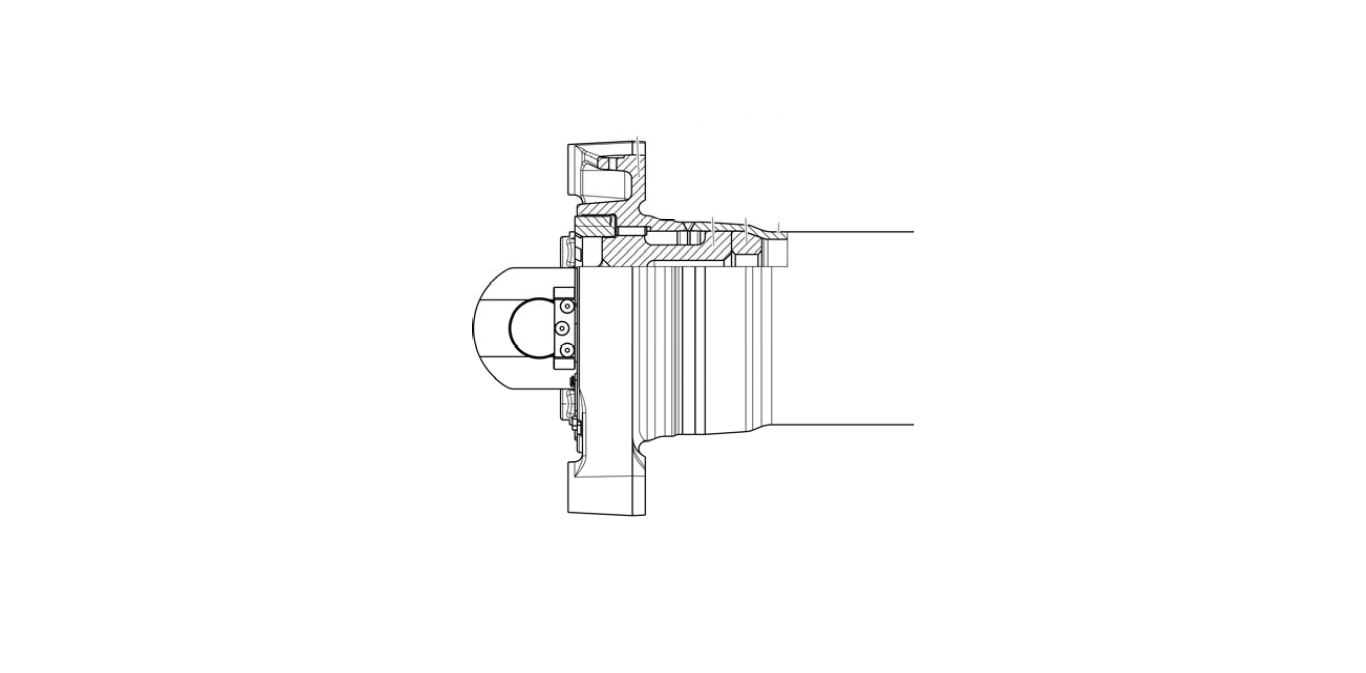
\includegraphics[width = 0.9\textwidth]{VRohr}};
\node (A) at (0,3) {\textbf{A}};
\draw[thick] (-2.8,1.65) -- (A);
%\node (B) at (0,-2.4) {A};
%\draw (-3.4,-2.15) -- (B);
\end{tikzpicture}
\caption{Schienenfahrzeugkomponente f\"ur Aufgabe \ref{Ta:Welding}}
\label{Fig:VRohr}
\end{center}
\end{figure}


\question
\label{Ta:Welding}
In Abbildung \ref{Fig:VRohr} wird das Verfromungsrohr einer automatischen Kupplung eines Nahverkehrstriebzugs dargestellt, die Schwei{\ss}naht wird nur bei Drucklasten \"uber den Druckring (4) belastet.

Es handelt sich um eine V-Naht, die aus konstruktiven Gr\"unden einseitig durchgeschwei{\ss}t wird und bei der keine Badsicherung m\"oglich ist.

\begin{table}[htdp]
\caption{default}
\begin{center}
\begin{tabular}{|c|c |c |c |}
\hline
\multirow{2}{*}{Beanspruchungszustand} & \multicolumn{3}{|c|}{Sicherheitsbed\"urfnis} \\ \cline{2-4}
 & Hoch & Mittel & Niedrig \\ \hline
Hoch & CP A & CP B & CP C2 \\ \hline
Mittel & CP B & CP C2 & CP C3 \\ \hline
Niedrig & CP C1 & CP C3 & CP D \\ \hline 
\end{tabular}
\caption{Tabelle Beanspruchungszustand und Sicherheitsbed\"urfnis}
\end{center}
\label{default}
\end{table}%

\begin{table}[htdp]
\caption{default}
\begin{center}
\begin{tabular}{|c|c|}
\hline
\multirow{2}{*}{Schwei{\ss}nahtg\"uteklasse} & Schwei{\ss}nahtpr\"ufklasse \\
& (Mindestanforderung) \\ \hline 
 CP A & CT 1 \\ \hline
 CP B & CT 2 \\ \hline
 CP C1 & CT 2 \\ \hline
 CP C2 & CT 3 \\ \hline
 CP C3 & CT 4 \\ \hline
 CP D & CT 4 \\ \hline
\end{tabular}
\caption{Tabelle G\"ute- und Pr\"ufklassem}
\end{center}
\label{default}
\end{table}%

\newpage
	\begin{parts}
	\part[4] Benennen Sie das Sicherheitsbed\"urfnis der mit \textbf{A} gekennzeichneten Schwei{\ss}naht und begr\"unden Sie.
	\makeemptybox{\stretch{1}}
	\part[4] Welche Schwei{\ss}nahtg\"ute- und Pr\"ufklasse ergibt sich bei geringer Beanspruchung?
	\makeemptybox{\stretch{1}}
	\newpage
	\begin{figure}[htbp]
	\begin{center}
	\includegraphics[width = 0.35\textwidth]{MKJ} \\
	\includegraphics[width = 0.95\textwidth]{Bauform}
	\end{center}
	\caption{MKJ-Diagramm und Bauformen\"ubersicht aus der DVS 1612 (Auszug)}
	\label{Fig:MKJ}
	\end{figure}

	%\newpage
	\part[4] Ermitteln Sie die Kerbfalllinie und die zul\"assige Normalspannung aus Abbildung \ref{Fig:MKJ}. Markieren Sie im Diagramm (Abbildung \ref{Fig:MKJ}) und erl\"autern Sie Ihre Wahl.
	\makeemptybox{\stretch{1}}
	
	\end{parts}
\newpage
\section{Schrauben}
\label{Ta:Bolt}
\begin{figure}[htbp]
\begin{center}
\begin{tikzpicture}
\node (myfirstpic) at (0,0) {\includegraphics[width = 0.9\textwidth]{Plunger}};
\node (B) at (-2,4) {\textbf{B}};
\draw[thick] (1,3) -- (B);
%\node (B) at (0,-2.4) {A};
%\draw (-3.4,-2.15) -- (B);
\end{tikzpicture}
\caption{Schienenfahrzeugkomponente f\"ur Aufgabe \ref{Ta:Bolt}}
\label{Fig:Plunger}
\end{center}
\end{figure}


\question
Die in Abbildung \ref{Fig:Plunger} mit \textbf{B} markierten Schrauben verbindet die Anlenk\"ose mit der gashydraulischen Patrone und der Zugstange. Bei Aufbringung von Druckkr\"aften wird das Geh\"ause von innen mit Druck beaufschlagt (der von den Schrauben gehalten wird), bei Zugkr\"aften \"ubertragen die Schrauben diese.
\newpage
\begin{parts}
 \part[4] Weisen Sie der Verschraubung eine Risikoklasse gem\"a{\ss} DIN 25201 zu. Begr\"unden Sie.
 \makeemptybox{\stretch{1}}
% \newpage
 \part[4] Bei der Routinepr\"ufung weisen einige Schrauben eine reduzierte Klemmkraft auf. Stellen Sie eine Vermutung \"uber die Ursache an.
 \makeemptybox{\stretch{1}}
\part[4] Wie w\"urden Sie die betrachtete Schraubverbindung robuster gegen Setzeffekte gestalten?
 \makeemptybox{\stretch{1}}
 \end{parts}

%%%%
\newpage
%\section*{Projektplanung und -dokumentation}
%Betrachten Sie als Beispielprojekt die Erstellung einer Abschlussarbeit am Lehrgebiet Schienenfahrzeugtechnik. Das Projekt besteht aus folgenden Einzelschritten, jeweils mit Vorg\"anger sowie Dauer in Arbeitstagen im Format (Pre/Dur):
%	\begin{enumerate}
%		\item \label{En:KickOff} Beginn der Bearbeitung (-/Meilenstein)
%		\item \label{En:LR} Literaturrecherche (\ref{En:KickOff}/90)
%		\item \label{En:PV} Planung und Vorbereitung (\ref{En:KickOff}/$\mathbf{x}$)
%		\begin{enumerate}
%		\item \label{En:A} Eingrenzen der Problemstellung (\ref{En:KickOff}/5)
%		\item \label{En:B} Erarbeiten der Fragestellung (\ref{En:A}/5)
%		\item \label{En:C} Review mit Betreuer (\ref{En:B}/Meilenstein)
%		\item \label{En:D} Formulieren der Ziele und Hypothese (\ref{En:C}/10)
%		\item \label{En:E} Ermitteln und Beschreiben des Forschungsstands (\ref{En:D}/5)
%		\item \label{En:F} Darstellung von Methode und Material (\ref{En:D}/2)
%		\item \label{En:G} Erstellung eines Gliederungsentwurfs (\ref{En:D}/1)
%		\item \label{En:H} Entwurf eines Literaturverzeichnisses(\ref{En:D}/1)
%		\item \label{En:I} Erstellung eines groben Zeitplans (\ref{En:D}/1)
%		\item \label{En:J} Review mit Betreuer (\ref{En:F}, \ref{En:G}, \ref{En:H}, \ref{En:I}/Meilenstein)
%	\end{enumerate}
%		\item \label{En:K} Durchf\"uhrung der Forschungsarbeit (\ref{En:J}/$\mathbf{y}$)
%		\begin{enumerate}
%			\item \label{En:L} Datenerhebung (\ref{En:K}/10)
%			\item \label{En:M} Analyse der Daten (\ref{En:L}/5)
%			\item \label{En:N} Modellbildung (\ref{En:M}/15)
%			\item \label{En:O} Modellvalidierung (\ref{En:N}/15)
%			\item \label{En:P} Review mit Betreuer (\ref{En:O}/Meilenstein)
%		\end{enumerate}
%		\item \label{En:R} Erstellung Abschlussarbeit(\ref{En:P}/$\mathbf{z}$)
%	\end{enumerate}
%Die gesamte Bearbeitungszeit betr\"agt 20 Wochen mit je 5 Arbeitstagen.
%\newpage
%\question
%\begin{parts}
%	\part[10] Erstellen Sie eine Work Breakdown Structure des Projekts und vermerken Sie an jedem Teilschritt die Dauer des Teilschritts.
%	\makeemptybox{\stretch{1}}
%%	\newpage
%%	\part[10] Stellen Sie den Projektablauf in Form einer Design Structure Matrix dar. Bilden Sie Cluster.
%%	\makeemptybox{\stretch{2}}
%	\part[8] Nutzen Sie die Vorlage auf der Folgeseite, um unter der Voraussetzung der Bearbeitung durch einen Studierenden ein Gantt-Diagramm f\"ur das Projekt zu erstellen.
%	\newpage
%	\begin{landscape}
%\begin{center}
%\tiny
%%\bgroup
%%\def\arraystretch{0.9} 
%\begin{tabular}{|l|c|c|c|c|c|c|c|c|c|c|c|c|c|c|c|c|c|c|c|c|c|c|}
%\hline
%Action Item & Pre & Dur & 01 & 02 & 03 & 04 & 05 & 06 & 07 & 08 & 09 & 10 & 11 &12 &13 & 14 & 15& 16 & 17 & 18 & 19 & 20\\ \hline 
%& & & & & & & & & & & & & & & & & & & & & &\\[5pt] \hline 
%& & & & & & & & & & & & & & & & & & & & & &\\[5pt] \hline 
%& & & & & & & & & & & & & & & & & & & & & &\\[5pt] \hline 
%& & & & & & & & & & & & & & & & & & & & & &\\[5pt] \hline 
%& & & & & & & & & & & & & & & & & & & & & &\\[5pt] \hline 
%& & & & & & & & & & & & & & & & & & & & & &\\[5pt] \hline 
%& & & & & & & & & & & & & & & & & & & & & &\\[5pt] \hline 
%& & & & & & & & & & & & & & & & & & & & & &\\[5pt] \hline 
%& & & & & & & & & & & & & & & & & & & & & &\\[5pt] \hline 
%& & & & & & & & & & & & & & & & & & & & & &\\[5pt] \hline 
%& & & & & & & & & & & & & & & & & & & & & &\\[5pt] \hline 
%& & & & & & & & & & & & & & & & & & & & & &\\[5pt] \hline 
%& & & & & & & & & & & & & & & & & & & & & &\\[5pt] \hline 
%& & & & & & & & & & & & & & & & & & & & & &\\[5pt] \hline 
%& & & & & & & & & & & & & & & & & & & & & &\\[5pt] \hline 
%& & & & & & & & & & & & & & & & & & & & & &\\[5pt] \hline 
%& & & & & & & & & & & & & & & & & & & & & &\\[5pt] \hline 
%& & & & & & & & & & & & & & & & & & & & & &\\[5pt] \hline 
%& & & & & & & & & & & & & & & & & & & & & &\\[5pt] \hline 
%& & & & & & & & & & & & & & & & & & & & & &\\[5pt] \hline 
%& & & & & & & & & & & & & & & & & & & & & &\\[5pt] \hline 
%& & & & & & & & & & & & & & & & & & & & & &\\[5pt] \hline 
%& & & & & & & & & & & & & & & & & & & & & &\\[5pt] \hline 
%& & & & & & & & & & & & & & & & & & & & & &\\[5pt] \hline 
%& & & & & & & & & & & & & & & & & & & & & &\\[5pt] \hline 
%& & & & & & & & & & & & & & & & & & & & & &\\[5pt] \hline 
%& & & & & & & & & & & & & & & & & & & & & &\\[5pt] \hline 
%& & & & & & & & & & & & & & & & & & & & & &\\[5pt] \hline 
%& & & & & & & & & & & & & & & & & & & & & &\\[5pt] \hline 
%& & & & & & & & & & & & & & & & & & & & & &\\[5pt] \hline 
%& & & & & & & & & & & & & & & & & & & & & &\\[5pt] \hline 
%& & & & & & & & & & & & & & & & & & & & & &\\[5pt] \hline 
%%& & & & & & & & & & & & & & & & & & & & & &\\[5pt] \hline 
%%& & & & & & & & & & & & & & & & & & & & & &\\[5pt] \hline 
%\end{tabular}
%\end{center}
%Kommentare:
%\makeemptybox{\stretch{1}}
%\end{landscape}
%	\newpage
%	\part[6] Markieren Sie den kritischen Pfad im Gantt-Diagramm. 
%	
%	Kommentare:
%\makeemptybox{\stretch{1}}
%%	\part[6] Benennen Sie f\"ur $\mathbf{x}$, $\mathbf{y}$ sowie $\mathbf{z}$ die minimale Dauer, jeweils unter der Annahme eines Beabeiters bzw. unendlich vieler Bearbeiter, wobei jeder Einzelschritt nicht weiter aufgeteilt werden kann.
%%\makeemptybox{\stretch{1}}
%\end{parts}
\newpage
\section{Projektplanung und -dokumentation}
Betrachten Sie als Beispielprojekt die Erstellung einer Parkbahn-Lokomotive f\"ur die IMechE \textit{Railway Challenge}. Gem\"a{\ss} derzeitiger Planung besteht das Projekt aus folgenden Einzelschritten, jeweils mit Vorg\"anger sowie Dauer in Monaten im Format (Vorg\"anger/Dauer) sowie einem evtl. notwendigen zeitlichen Abstand zum Vorg\"anger:
	\begin{enumerate}
		\item Gruppe Design
		\begin{enumerate}
		\item Kickoff (-/Meilenstein)
		\item Grobkonzept (1a/1)
		\item Interface Freeze (1b/Meilenstein)
		\item Detailkonstruktion (1c/2)
		\item Review (1b + 1 Monat/Meilenstein)
		\item Design Freeze (1c/Meilenstein)
		\end{enumerate}
		\item Gruppe Beschaffung, Montage
		\begin{enumerate}
		\item Beschaffung (1f/3)
		\item Montage (1f + 2 Monate/1)
		\end{enumerate}
		\item Gruppe Doku, Software, Optimierung
		\begin{enumerate}
		\item Software (2b/4)
		\item Dokumentation (2b + 2 Monate/1)
		\item Optimierung (2b + 3 Monate/2)
		\end{enumerate}
	\end{enumerate}

%\newpage
\question
\begin{parts}
	\part[10] Nutzen Sie die Vorlage, um unter der Voraussetzung der Bearbeitung durch ein beliebig gro{\ss}es Projekteam ein Gantt-Diagramm f\"ur das Projekt zu erstellen.
	\begin{center}
            		\begin{ganttchart}[vgrid, hgrid, 
		%today = 4, 
		%progress=today,
		%progress label text=\relax,
		%today=3,
		x unit = 7mm,
		y unit chart = 6 mm,
		bar/.append style={fill=blue!80!black},
		chart element start border=right,
		 bar/.append style={fill=none, draw = none},
		milestone/.append style={fill=none, draw = none},
		group/.append style={fill=none, draw = none}
		]{1}{13}
			\gantttitle{Railway Challenge}{13} \\
			\gantttitlelist{1,...,13}{1}\\
			\ganttgroup{Design}{1}{4} \\
			\ganttmilestone{Kick Off}{1}\\
			\ganttbar{Grobkonzept}{1}{2} \\
			\ganttmilestone{Interface Freeze}{2}\\
			\ganttbar{Detailkonstruktion}{2}{4} \\
			\ganttmilestone{Review}{3}\\
			\ganttmilestone{Design Freeze}{4}\\
			\ganttgroup{Beschaffung, Montage}{4}{7} \\
			\ganttbar{Beschaffung}{4}{7} \\
			\ganttbar{Montage}{6}{7} \\
			\ganttgroup{Doku, Software, Optimierung}{7}{12} \\
			\ganttbar{Software}{7}{11} \\
			\ganttbar{Dokumentation}{9}{10} \\
			\ganttbar{Optimierung}{10}{12} \\
			\ganttmilestone{Challenge}{12}
%			\ganttlink{elem1}{elem2}
%			\ganttlink{elem1}{elem5}
%			\ganttlink{elem2}{elem3}
%			\ganttlink{elem3}{elem4}
%			\ganttlink{elem4}{elem6}
%			\ganttlink{elem4}{elem6}
%			\ganttlink{elem5}{elem6}
			\end{ganttchart}
        		\end{center}
	Kommentare (optional):
\makeemptybox{\stretch{1}}

\newpage

	\part[4] Markieren Sie den kritischen Pfad im Gantt-Diagramm auf der Folgeseite und geben Sie die L\"ange des kritischen Pfades an. 
\makeemptybox{\stretch{1}}
	\part[4] Welche Risiken sehen Sie im Projektablauf? Durch welche Ma{\ss}nahmen lassen sich diese Risiken vermindern?
\makeemptybox{\stretch{1}}
%	\part[6] Benennen Sie f\"ur $\mathbf{x}$, $\mathbf{y}$ sowie $\mathbf{z}$ die minimale Dauer, jeweils unter der Annahme eines Beabeiters bzw. unendlich vieler Bearbeiter, wobei jeder Einzelschritt nicht weiter aufgeteilt werden kann.
%\makeemptybox{\stretch{1}}
\end{parts}
\end{questions}
\end{document}